\documentclass[xcolor=dvipsnames]{beamer}
\usepackage[utf8]{inputenc}
\usepackage[slovak]{babel}
\usepackage{graphics}
\usepackage{color}
\usepackage{amsfonts}
\usepackage{wrapfig}
\usepackage{tikz}
\usepackage[export]{adjustbox}

\usetheme{PaloAlto}
\useinnertheme{rounded}
\beamertemplatenavigationsymbolsempty
\setbeamertemplate{footline}[frame number]
\newcommand{\myuv}[1]{\quotedblbase #1\textquotedblleft}
 
 
%Information to be included in the title page:
\title{Zabezpečení dat pomocí 16/32-bit. kódu CRC (ARM/FITkit3)}
\subtitle{Mikroprocesorové a vestavěné systémy} 
\author{Dávid Bolvanský}
\institute{Vysoké učení technické v Brně \\Fakulta informačních technologií}
 
 
 
\begin{document}
 
\frame{\titlepage}

\begin{frame}
\frametitle{Obsah}
\tableofcontents
\end{frame}

\section{Zadanie projektu}
 
\begin{frame}
\frametitle{Zadanie projektu}
\begin{itemize}
\item projekt pre ARM/FITkit3
\item vytvoriť vhodný blok dát na zabezpečenie pomocou CRC
\item zabezpečiť dáta pomocou CRC16/32 troma spôsobmi
\begin{itemize}
	\item pomocou hardvérového modulu Cyclic Redundancy Check (CRC) z čipu K60
	\item získaním CRC podľa polynómu z tabuľky
	\item výpočtom CRC podľa polynómu
\end{itemize}
\item zaniesť jednu či viac chýb do bloku dát
\item overiť schopnosti tejto metódy detegovať chyby
\end{itemize}
\end{frame}


\section{Riešenie}

\begin{frame}
\frametitle{Úvod do riešenia}
\begin{itemize}
\item použité Kinetis Design Studio 3.0 (Windows verzia) + SDK
\item interakcia s hardvérom -- CRC/UART -- pomocou SDK API
\item vytvorený blok dát -- reťazec obsahujúci text Lorem Ipsum
\end{itemize}
\end{frame}

\begin{frame}
	\frametitle{Výpočet CRC pre blok dát}
	\begin{itemize}
		\item výpočet CRC16/32 pomocou HW modulu (SDK API)
		\item výpočet CRC16/32 pomocou tabuľky s predvypočítanými hodnotami 
		\item výpočet CRC16/32 pomocou základného algoritmu
		\item overenie správnosti vypočítaného CRC porovnaním s predvypočítaným správnym CRC
	\end{itemize}
\end{frame}


\begin{frame}
	\frametitle{Zanesenie chýb, prezentovanie výsledkov}
	\begin{itemize}
		\item zanesená jedna chyba $\rightarrow$ nové výpočty CRC $\rightarrow$ nové porovnania
		\item zanesené viaceré chyby $\rightarrow$ nové výpočty CRC $\rightarrow$ nové porovnania
		\item prezentovanie výsledkov správnosti výpočtov CRC $\rightarrow$ UART $\rightarrow$ výstup na terminál
	\end{itemize}
\end{frame}

\begin{frame}
	\frametitle{Ukážka výstupu na terminál}
	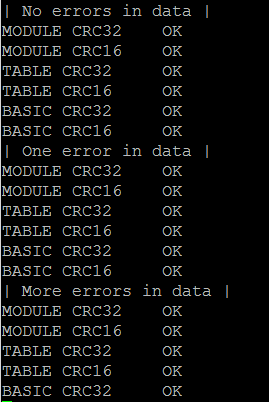
\includegraphics[width=6cm, height=\textheight]{crc.png}
\end{frame}

\begin{frame}
	\frametitle{Záver}
	\center{\Huge{Ďakujem za pozornosť.}}
\end{frame}
 
\end{document}


